\documentclass{article}
\usepackage[T1]{fontenc}
\usepackage{lmodern}
\usepackage{graphicx}
\usepackage{amsmath,amssymb}
\usepackage[a4paper,margin=2cm]{geometry}
\usepackage[absolute,overlay]{textpos}
\setlength{\TPHorizModule}{1mm}
\setlength{\TPVertModule}{1mm}
\usepackage[indonesian]{babel}
\usepackage{hyperref}
\setlength{\emergencystretch}{2em}
% unit: Halaman 65

\begin{document}

% === Halaman 65 (llm) ===

\vspace{180.87mm}

Museum Sandi di Yogyakarta (Sumber: http://museum.lemsaneg.go.id/)

\vspace{80mm}

Alamat Jl. Faridan Muridan Noto No. 21, Kota Baru, Yogyakarta. Ini museum san satu-satunya di Indonesia, bahkan di dunia. Di dalamnya terdapat berbagai koleksi alat sandi yang pernah digunakan di Indonesia

% deskripsi: Foto bangunan Museum Sandi di Yogyakarta dengan arsitektur kolonial dan halaman depan yang luas.
% bbox normalisasi: [0.2210, 0.1560, 0.7620, 0.7650]
\begin{textblock*}{113.61mm}(46.41mm,46.33mm)
\noindent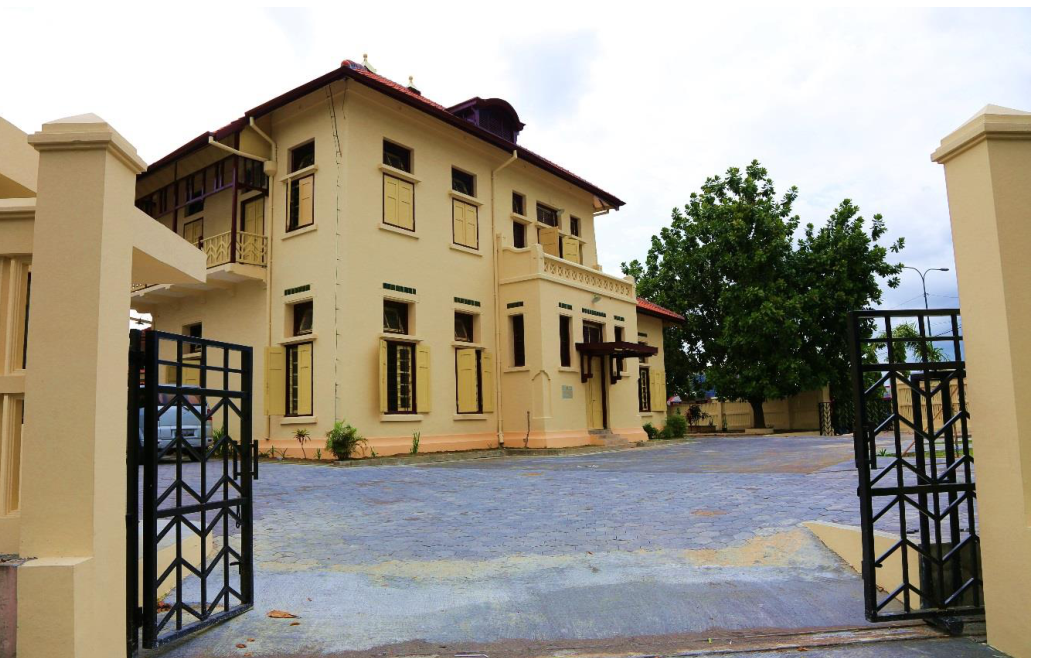
\includegraphics[width=113.61mm,height=180.87mm]{../../images/llm/page_065_img_01.png}%
\end{textblock*}

\end{document}
